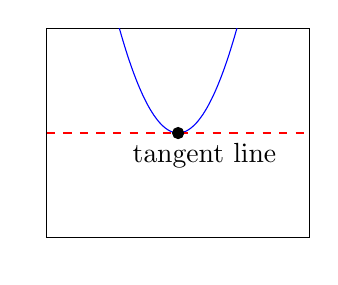
\begin{tikzpicture}
	\begin{axis}[
			axis lines        = box,
			xmin              = -5,
			xmax              = 5,
			ymin              = -5,
			ymax              = 5,
			xtick             = \empty,
			ytick             = \empty,
			xlabel            = \empty,
			ylabel            = \empty,
			trig format plots = rad,
			width             = 14em,
		]

		% it draws a vertical line if i don't do this
		\addplot [
			smooth,
			color=blue,
			samples=50,
		]{x^2};

		\addplot [
			color=black,
			mark=*
		]coordinates{(0, 0)};

		\draw [dashed, red] (-5, 0) -- (5, 0);

		\node[below] at (1, 0) {tangent line};
	\end{axis}
\end{tikzpicture}

